% !TeX root = ../dissertation.tex
\begin{sidewaysfigure}
	\centering

	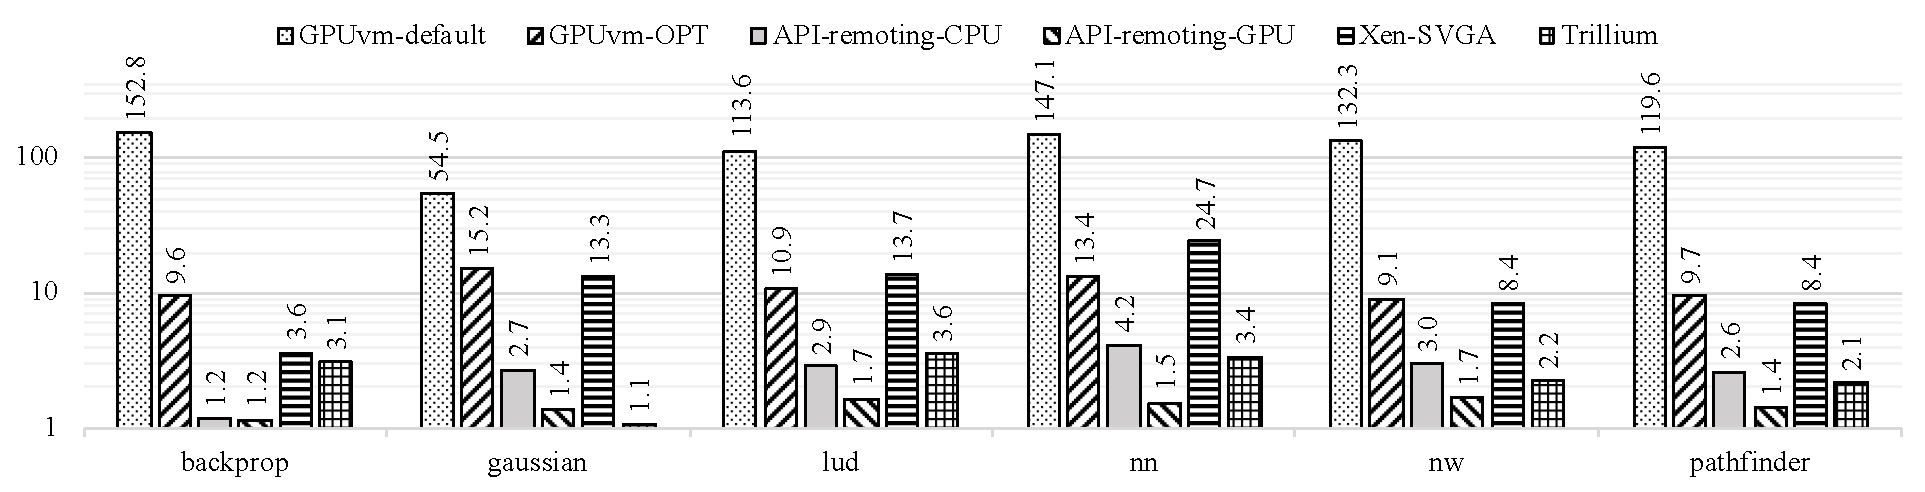
\includegraphics[width=\linewidth,clip]{trillium/data/cross_product_overhead_noRPC_OptInit.pdf}
	\caption{{\footnotesize End-to-end execution times of benchmarks on virtualization prototypes, relative to end-to-end execution time on the NVIDIA CUDA runtime in a native setting. gRPC overhead is removed from the reported measurements, which is up to 10\% of the total execution time for API remoting, and 40\% for \Trillium.}}
	\label{fig_all_overhead}

	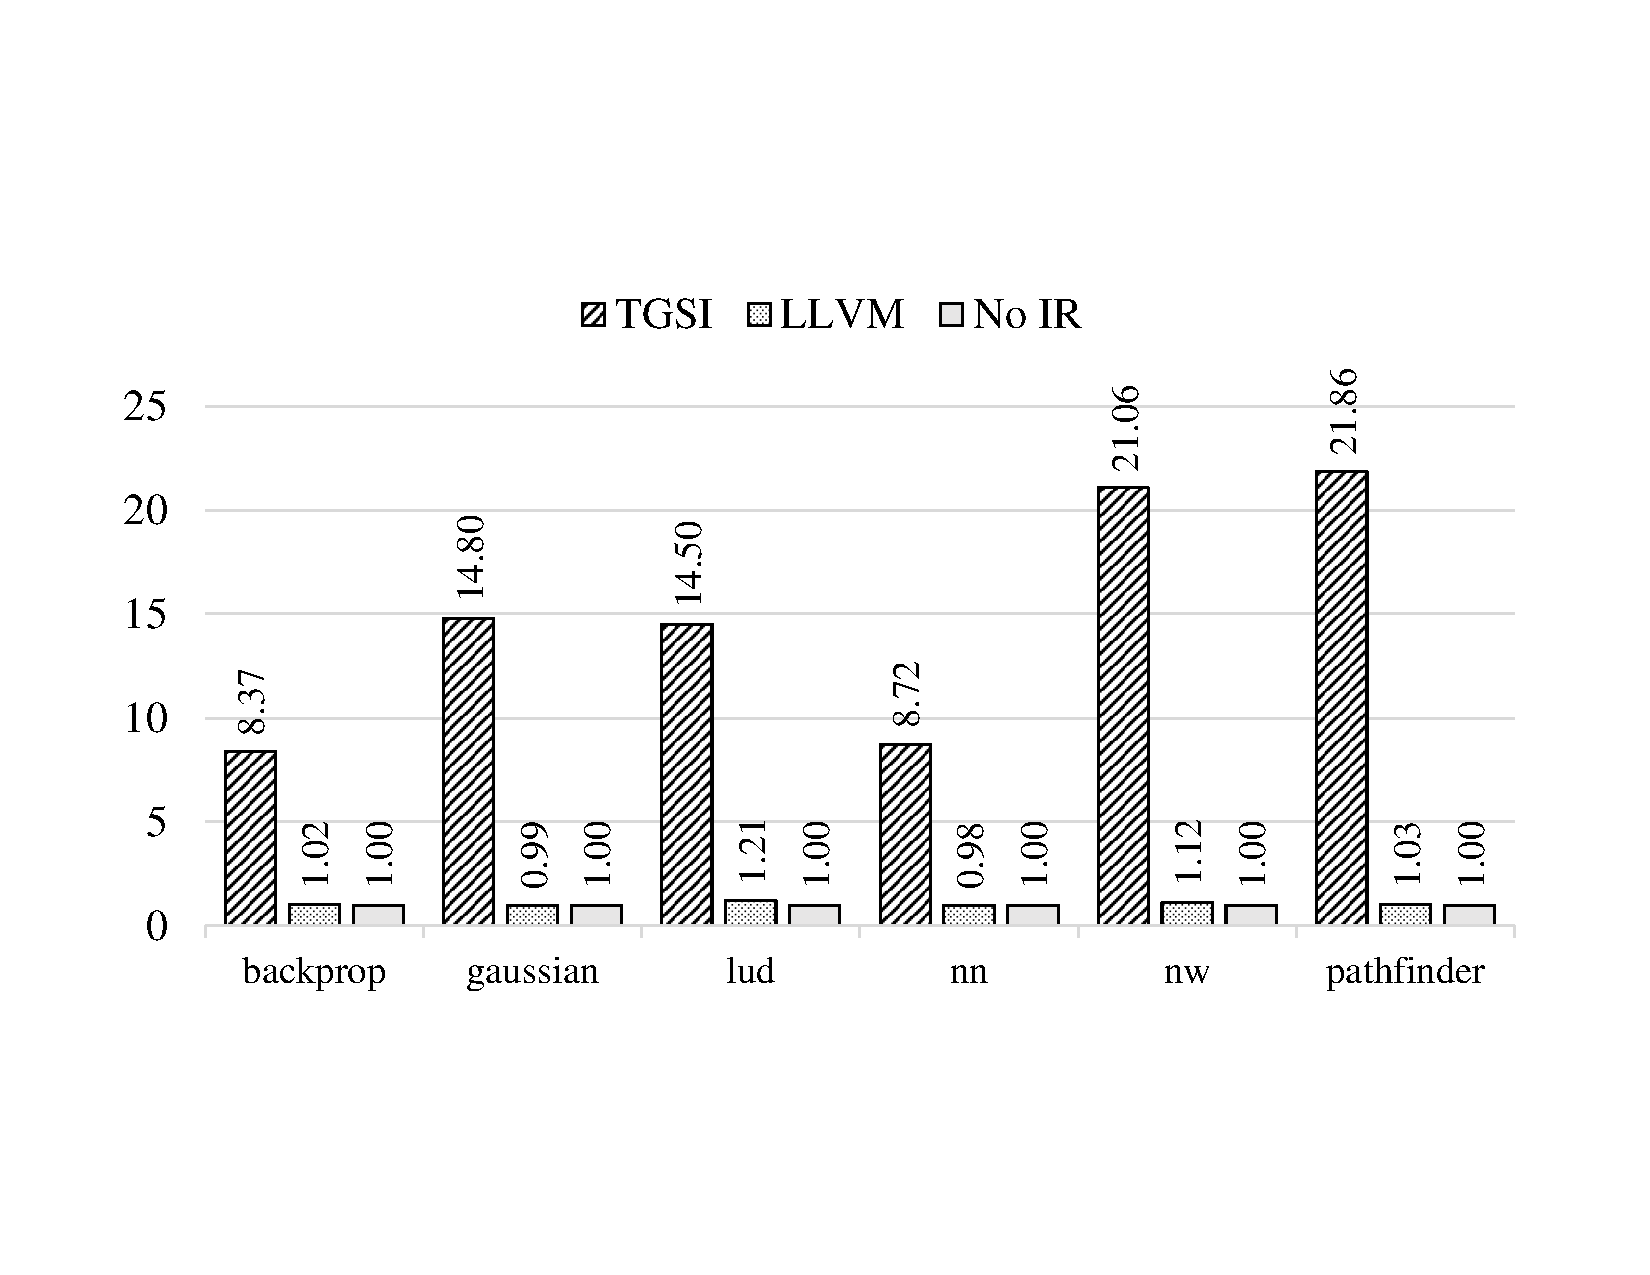
\includegraphics[width=.5\linewidth,trim={2cm 4.5cm 2cm 5cm},clip]{trillium/data/trillium/trillium_kernel.pdf}
	\caption{{\footnotesize Kernel execution slowdown due to virtual ISAs. TGSI: the LLVM TGSI back-end compiler used in \XenSVGA. LLVM: LLVM NVIDIA PTX (NVPTX) back-end used in \Trillium. No IR: native NVIDIA compiler.}}
	\label{fig_trillium_kernel}

\end{sidewaysfigure}

\section{Evaluation}
\label{sec:trilliumeval}

\subsection{End-to-End}
Figure~\ref{fig_all_overhead} depicts one of the major results from this
chapter: an end to end empirical analysis of systems representative of all of
prior canonical virtualization schemes. GPUvm~\cite{GPUvm} stands in for
full-virtual\-ization designs, in its default configuration (\gpuvmdef), and
in its fully optimized configuration (\gpuvmopt). \apigpu and \apicpu
represent user-space API remoting schemes, while \XenSVGA represents the SVGA
design. \Trillium is very similar to \XenSVGA, other than that it elides ISA
virtualization (the use of the TGSI vISA).

Figure~\ref{fig_all_overhead} shows the end-to-end execution time (relative to
native GPU execution) for the six chosen benchmarks for all the systems
evaluated. As expected, traditional API remoting designs incur the lowest
overhead, which is achieved by giving up hypervisor interposition.
\gpuvmopt exhibits about 9.1$\times$ slowdown for applications with
short-lived kernels (e.g. Needleman-Wunsh algorithm); the overhead can be as
high as 15.2$\times$ when the workload has long-running kernels (e.g. Gaussian
Elimination), proving that trap-based virtualization schemes are doomed to
squander the raw performance that makes accelerators desirable in the first
place. \XenSVGA fares better than \gpuvmdef and \gpuvmopt, but performs worse
than \apigpu, \Trillium, and in some cases even \apicpu. \XenSVGA is sensitive
to the performance lost in GPU kernel code resulting from redundant
compilation through TGSI (See Figure~\ref{fig_trillium_kernel} for deeper
analysis).

We find that remoting calls to a CPU is uniformly more performant than
full-virtualization of the GPU, and sometimes performs just as well as
(backprop) or better than remoting to the GPU (1.6$\times$ faster for the bfs
benchmark). The performance gain from accelerating the bfs kernel on the GPU
is severely dwarfed by the cost of initialization on the GPU). GPGPU compute
is only economical when it provides acceleration over the CPU; if overheads
make the CPU competitive, the profitability threshold has been crossed.
Further, the competitiveness of \apicpu suggests opportunity: systems could
back a virtual GPU with CPU if they can detect when it is profitable to do so.

Overall, it appears that user-space API remoting introduces the lowest
overhead when multiplexing Domain Specific Accelerators. However, the lack of
a viable interposition point means that the hypervisor is out of the loop and
can't make scheduling and resource allocation decisions, or ensure isolation.

\subsection{Impact of vISA choice}

Our hypothesis that ISA virtualization is redundant for GPGPUs (and DSAs
generally) is confirmed by the fact that \Trillium out performs \XenSVGA in
the empirical results presented in Figure~\ref{fig_all_overhead}. Deferring
the compilation of front-end code to the host not only eliminates redundant
translations, and the need to have a compiler in the guest driver, but also
ensures that the compiler used has a high-fidelity view of the physical
hardware.

Typically, DSA execution/compilation frameworks are tightly coupled with the
vISA used, making the choice of vISA even more tenuous as it leads to the
second order effect of having to rely on a particular implementation of the
compute framework (e.g., Mesa3D OpenCL vs NVIDIA OpenCL).

To understand the impact of the virtual ISA on the quality of the generated
GPU code, we measured GPU execution time for NVIDIA SASS kernels generated in
3 ways:
\begin{itemize}[nosep, topsep=0em, leftmargin=1em,labelwidth=*,align=left]
\item using the Mesa3d OpenCL stack (OpenCL$\rightarrow{}$TGSI$\rightarrow{}$SASS),
\item using the LLVM OpenCL stack (OpenCL$\rightarrow{}$LLVM IR$\rightarrow{}$SASS),
\item and using the native NVIDIA OpenCL compiler (OpenCL$\rightarrow{}$SASS).
\end{itemize}

These measurements are reported in Figure~\ref{fig_trillium_kernel}
relative to kernel execution time in a native setting. Code generated from
TGSI IR is dramatically slower in all cases than code generated by the NVIDIA
OpenCL framework. We observe slowdowns of up to 22$\times$, with a harmonic
mean of 13$\times$ across the 6 benchmarks that were optimized for evaluation.

While we predicted the basic trend these experiments show, we were surprised
by the magnitude of the difference. We found quality of the kernel generated
by the LLVM NVPTX compiler to be comparable to native, at least in terms of
execution time. This is unsurprising given recent efforts~\cite{gpucc} to
optimize the LLVM tool-chain for NVIDIA GPUs.